\chapter{Performance Evaluation}
\label{Chapter5}
\lhead{Chapter 5. \emph{Performance Evaluation}} % Write in your own chapter title to set the page header

In this chapter, we first will introduce our designed performance metrics in order to properly evaluate our proposed adaptive fanout \pp ~\gp. Then we will explain our simulation environment settings. Finally, we will analyze the simulation results.

\section{Performance Metrics}
As we stated in Section \ref{basic gossip}, the objective of our proposed approach is to achieve the balance between fast broadcasting time and long network lifetime. So obviously, the first two performance metrics that we proposed are \emph{Average \nl} and \emph{Average Message Broadcast Time}. Other performance metrics are \emph{Average Overhead Per Node Per Message}, \emph{Average Consumed Energy Per Node Per Message}, and \emph{Average Number of Success Broadcast Messages}.

\subsection{Average Network Lifetime}
%\textbf{Average Network Lifetime}

Before we define \emph{Average Network Lifetime}, we need to define \emph{Network Lifetime} first. 

\textbf{Network Lifetime}: The time duration which a wireless ad-hoc network can physically broadcast \msgs ~successfully.

When a \gn's energy is depleted, this \gn ~will no longer be able to transmit and receive new broadcast \msgs. Thus, this network is considered to be physically unable to broadcast \msgs ~successfully. Now the definition of \emph{Average Network Lifetime} is simply just an average over all \emph{Network Lifetime} under $n$ \gns ~case. For example, if we ran $s$ simulations under $n=10$ setting, and we denote \emph{Average Network Lifetime} for $10$ \gns ~as $L_{avg\_10}$, then the following equation can be used to calculate the \emph{Average Network Lifetime}.

\[ L_{avg\_10} =\frac{L_1 + L_2 + \ldots + L_{s}}{s} \]

This performance metric measures how long a wireless ad-hoc network with $n$ \gns ~can stay connected when running our proposed adaptive fanout \gp.

\subsection{Average Message Broadcast Time}
%\textbf{Average Message Broadcast Time}

Before we jump into the definition of \emph{Average Message Broadcast Time}, we first need to clearly define \emph{Message Broadcast Time}.

\textbf{Message Broadcast Time}: The maximum delay among \gns ~for each broadcast \msg.

Because here we are trying to measure the broadcast time of a certain \msg, it only makes sense when we sample the maximum delay among all \gns ~because the \msg ~received time of the last \gn ~determined our message broadcast time for a particular \msg. Now the \emph{Average Message Broadcast Time} is just an average over all \msg ~broadcast time under $n$ \gn ~case. Now because the randomness of our proposed \gp, each simulation under $n$ \gn ~case can result in different number of success broadcast \msgs. Therefore, for $n$ \gn ~case simulations, we first calculate the \emph{Average message broadcast time} for each simulation. And then we perform the average among those number to obtain this performance metrics data.

For example, let's denote the \emph{Average Message Broadcast Time} for $i$th simulation as $T_i$ and the \emph{Average Message Broadcast Time} for $n$ nodes as $T_{avg\_n}$. If we performed $s$ simulations, then the following equation can be used to calculate this metric:

\[ T_{avg\_n} = \frac{T_1 + T_2 + \ldots + T_s}{s} \]

This metric indicates the time needed for a broadcast \msg ~to reach every \gn ~in the network.

\subsection{Average Overhead Per Node Per Message}

The \emph{overhead} here is defined as the total number of packets sent by a \gn. These packets includes Ack packet, Request packet, and Data packet. For every simulation, in order to accurately measure the overhead for each \gn ~and for each broadcast \msg, we simply performed an average over $n$. And then take that number and further average over number of broadcast \msgs being sent. So for $k$th simulation, if we denote the overhead of node $i$ for \msg ~$j$ as $O_{ij}$, the number of \gns ~are $n$, and the system broadcast $m$ \msgs. Then for this simulation, the \emph{Average Overhead Per Node Per Message} can be computed using the following equation:

\[ O_{k} = \frac{(O_{11} + O_{21} + \ldots + O_{n1})  + \ldots + (O_{1m} + O_{2m} + \ldots + O_{nm})}{n\times m} \]

If we performed $s$ simulations under $n$ \gns ~setting, then the \emph{Average Overhead Per Node Per Message} among these simulations is:

\[ O_{avg\_n} = \frac{O_1 + O_2 + \ldots + O_s}{s} \]

%+ (O_{12} + O_{22} + \ldots + O_{n2})
%\mbox{Average Overhead Per Node Per Message}

This performance metric indicates how many packets are sent out for a \gn ~to facilitate broadcasting one \msg. 

\subsection{Average Energy Consumption Per Node Per Message}

This performance metric is quite self-explanatory. We measure the amount of energy consumed by each \gn ~during the simulation. For each simulation, first we average among every \gn's energy consumption. Then we take that number and average among $m$ \msgs. If we denote $E_k$ as the \emph{Average Energy Consumption Per Node Per Message} for the $k$th simulation under $n$ \gns. Then 

\[ E_k = \frac{E_{node\_1} + E_{node\_2} + \ldots + E_{node\_n}}{n\times m} \]

Now if we ran $s$ simulations, then \emph{Average Energy Consumption Per Node Per Message} under $n$ \gns ~can be calculated using the following equation:

\[ E_{avg\_n} = \frac{E_1 + E_2 + \ldots + E_s}{s} \]

This metric measures the amount of energy needed for a \gn ~to facilitate broadcasting one \msg. 

\subsection{Average Number of Broadcast Messages}

This metric measures how many \msgs ~can be successfully broadcast with limited energy sources. If we ran $s$ simulations under $n$ \gns ~setting, this metric can be computed using the following equation:

\[ N_{avg\_n} = \frac{N_1 + N_2 + \dots + N_s}{s} \]

\section{Simulation Environment Settings}

\wf ~speed among \gns: 1Mbps
\wf ~speed between the \sn ~and a \gn: 11Mbps
Gossip node maximum \wf ~range: 50m
Number of nodes: 10, 50, 90, 130, 170
Simulation stop time = 100000.0s
Initial battery energy = 108.0J
Gossip interval: 1.0s
Request interval 5.0s

In summary, the simulation parameters are set to be as follows:
\begin{itemize}
	\item Number of Nodes = 10, 20, 30, … , 200
	\item Simulation time = large enough to ensure energy depletion happens first
	\item Maximum Wifi Range = 50m
	\item Initial Energy = 108J
	\item Gossip Interval = 1.0s
	\item Solicit interval = 5.0s 
\end{itemize}

The number of nodes, simulation time, maximum wifi range, initial battery energy, gossip interval, and solicit interval are all the parameters I could control in the simulation. The number of nodes is ranging from 10 to 200 with step 10. The simulation time is set to be large enough to ensure any node's battery will die before the simulation stops. The maximum wifi range is set to be 50 meters so that no one node is connected to all other nodes. The initial battery energy is set to be 1080 Joule (equivalent to 100mAh) for every node. The gossip interval is set to be 1 second meaning for any node every second the gossip process will wake up and check if it need to gossip a new packet to its neighbors. The solicit interval is set to be 5 seconds which means every 5 seconds, a node will randomly pick a neighbor and query for their latest received packet. 

The simulation will stop when any node's energy was depleted. For each scenario (e.g. n = 10), 100 independent trials were simulated in order to gather performance data. Any simulation parameters other than number of nodes stay the same through all simulation trials. 



It should be noted that due to time limitations each topology file was only simulated once. Finally, we did statistical analysis upon those collected data.



\section{Results Analysis}

For cases of \emph{Fanout} $f=1$, we performed total of ?? simulations with number of \gns ~ranging from 10 to 170.

$f=1,5,10$  $f=adaptive$
insert a table here

success simulation
total simulation 

Fanout of gossip protocol is defined as the number of neighbors a node contact each time when a new packet is received. It is one of the parameters that control the behavior of gossip protocol. In one scenario, fanout is set to be one. In another scenario, fanout is set to be five. These two scenarios 's trials are conducted to compare to the adaptive fanout scenario. 

\begin{figure}
	\centering
	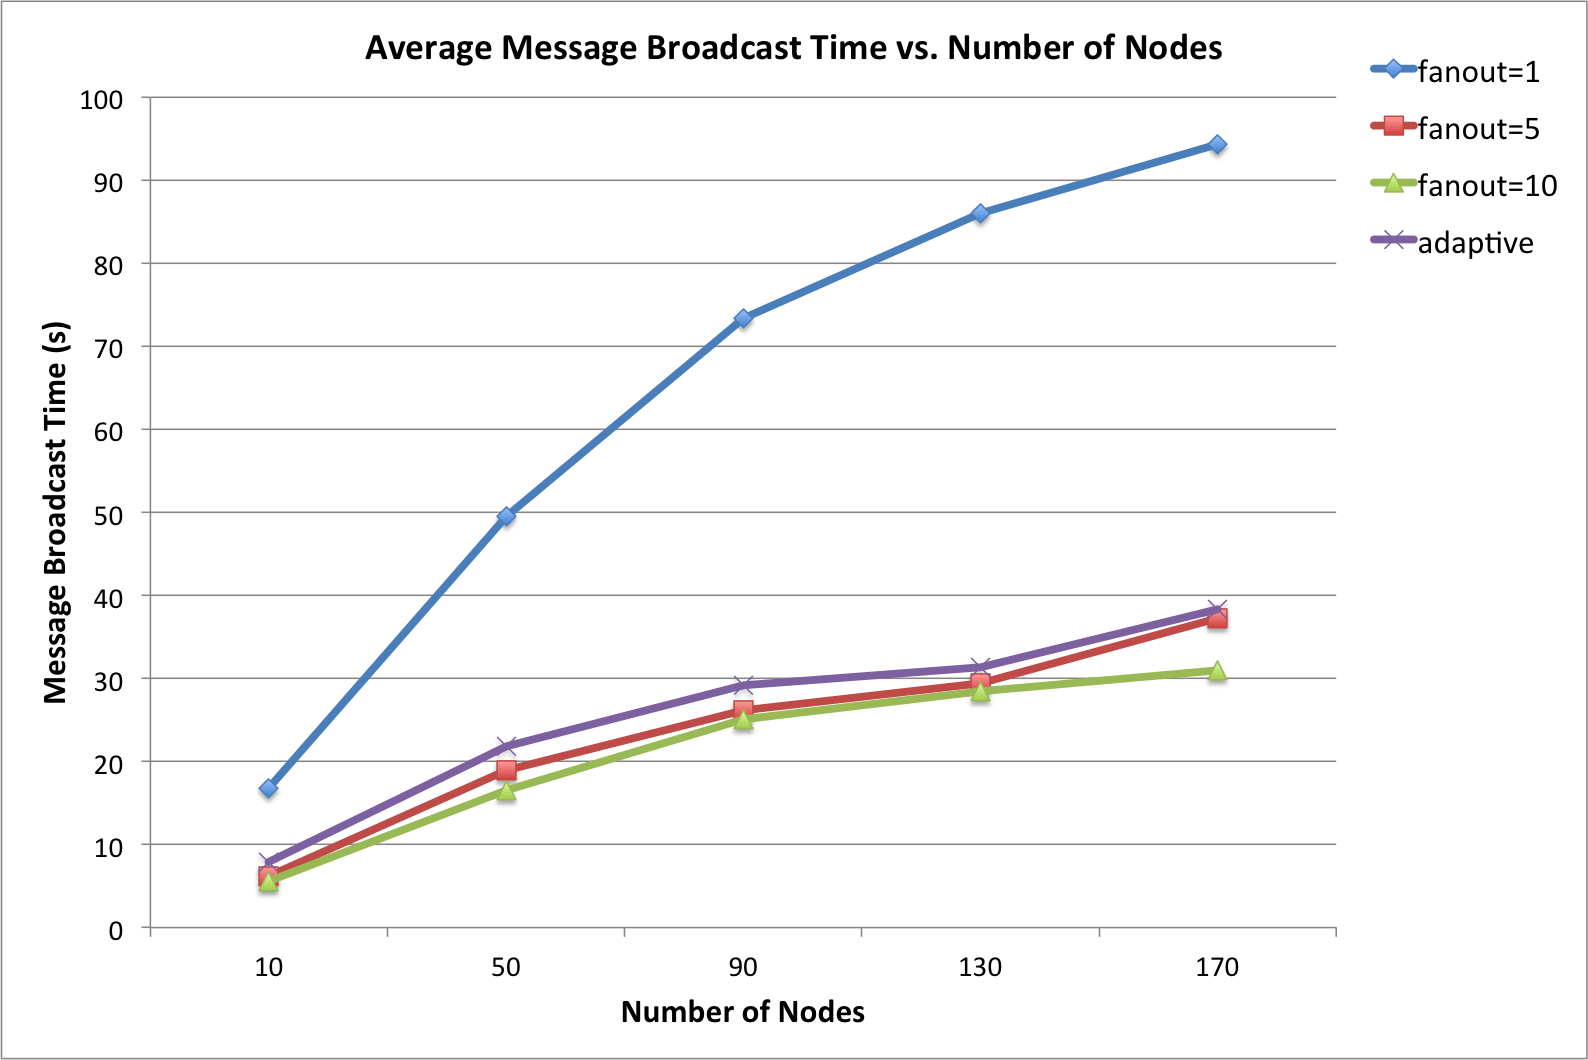
\includegraphics[width=5.5in]{brTime.png}
	\caption{Average message broadcast time vs. number of nodes}
	\label{fig:brTime}
\end{figure}

\begin{figure}
	\centering
	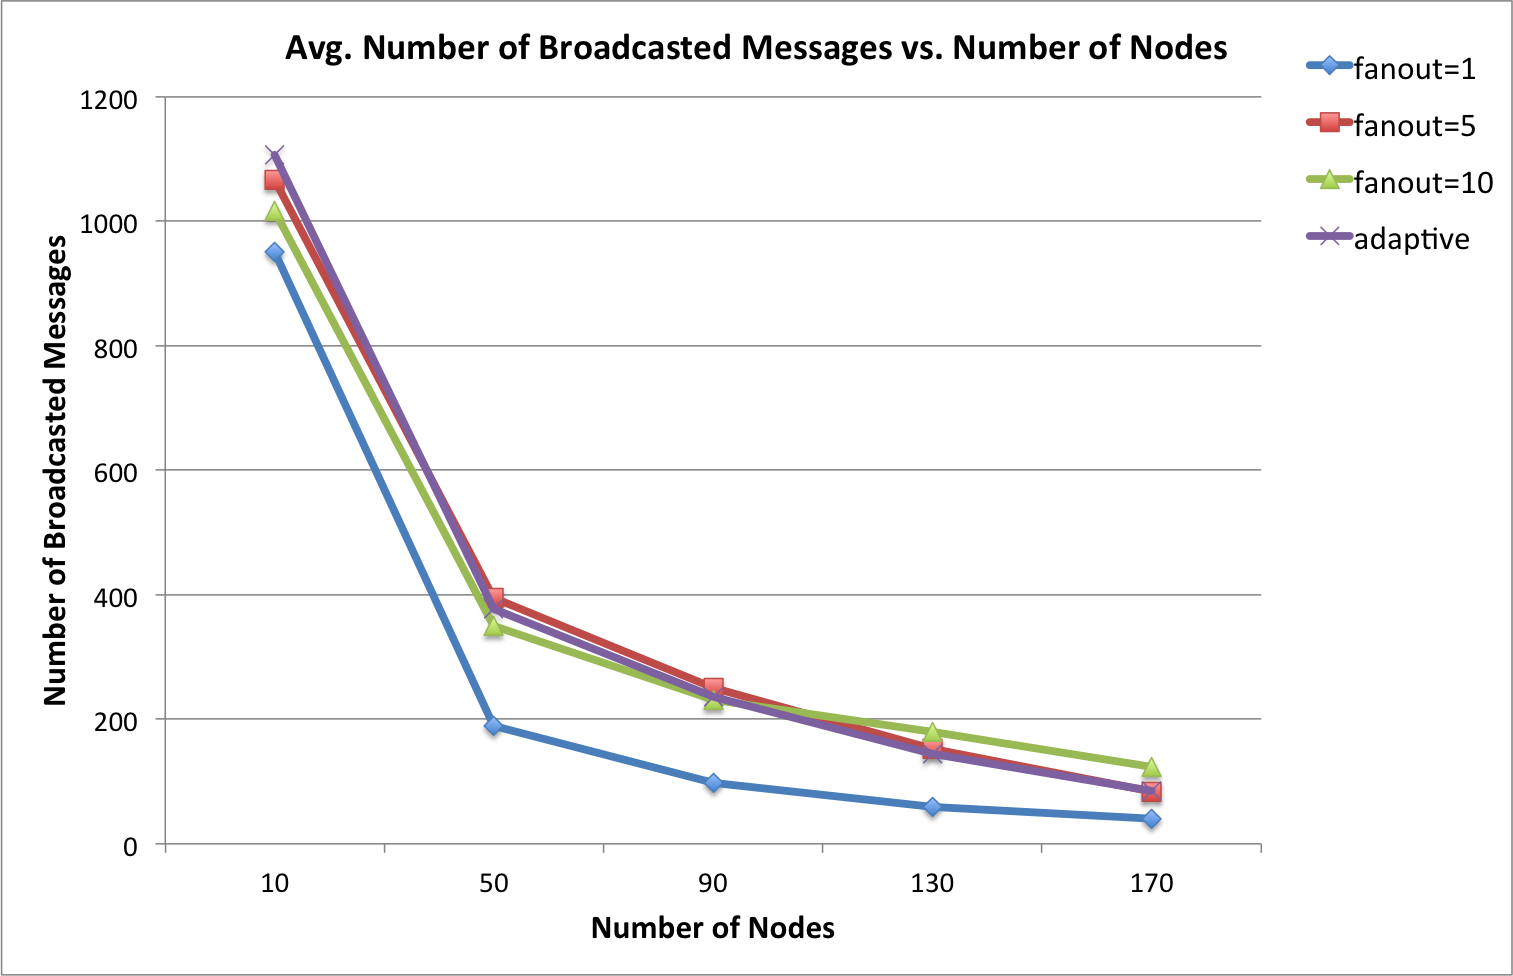
\includegraphics[width=5.5in]{brNum.png}
	\caption{Average number of broadcasted messages vs. number of nodes}
	\label{fig:brNum}
\end{figure}

\begin{figure}
	\centering
	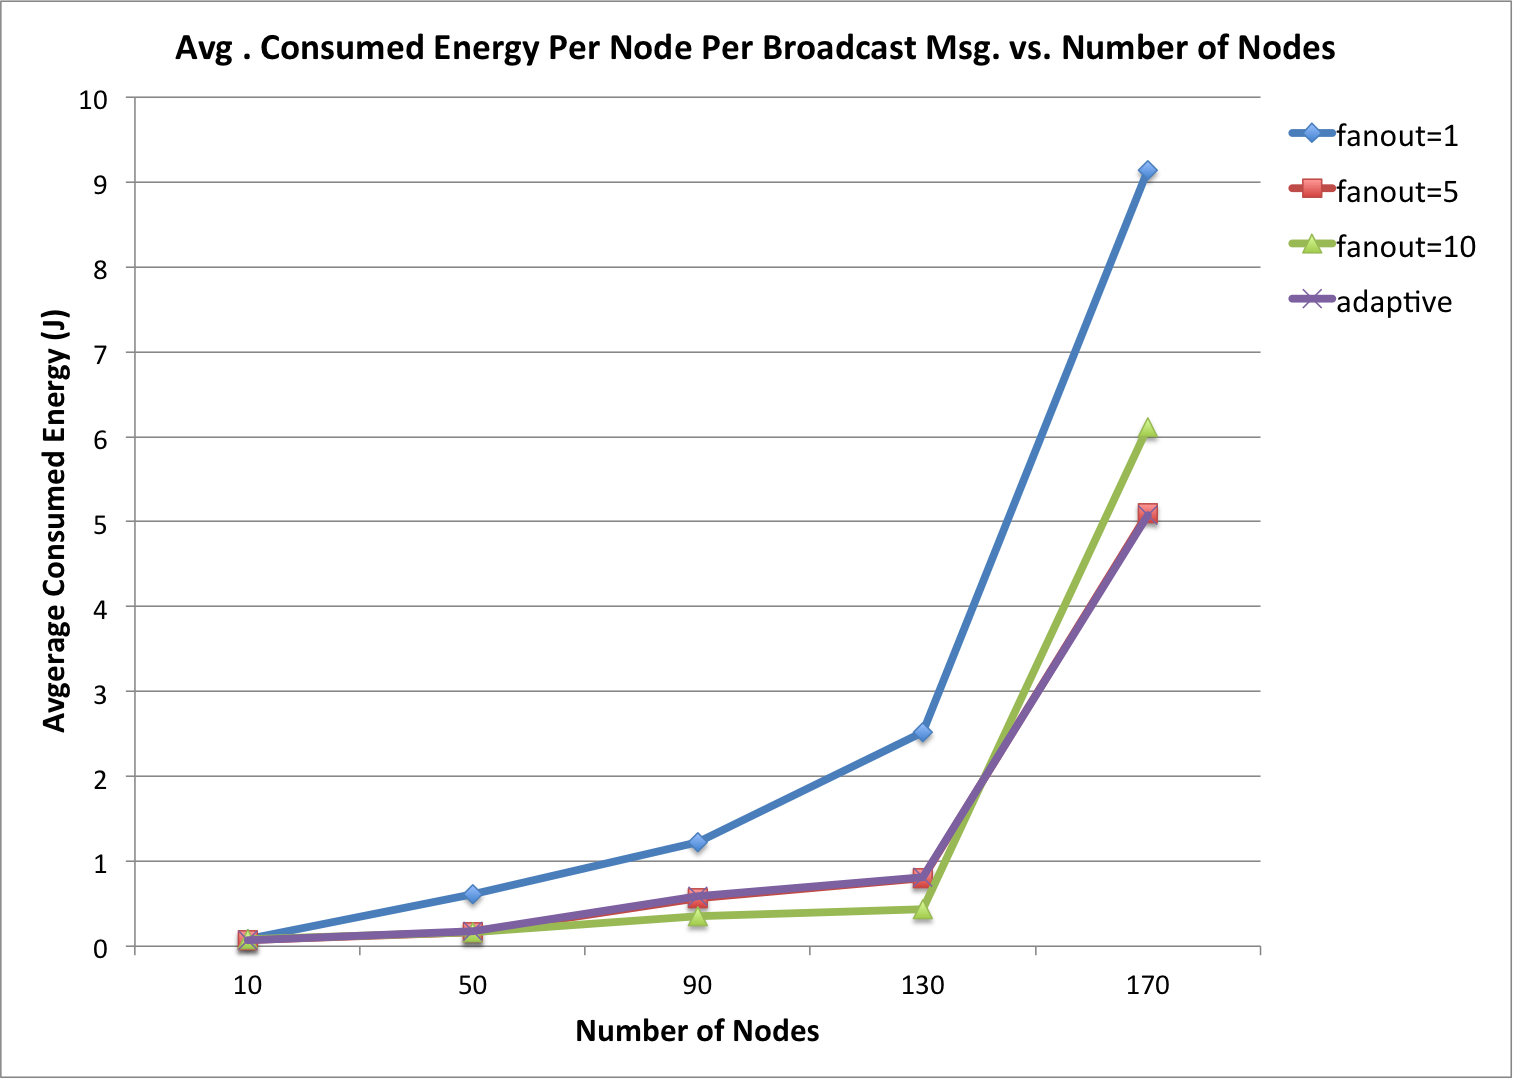
\includegraphics[width=5.5in]{energy.png}
	\caption{Average consumed energy per node per message vs. number of nodes}
	\label{fig:energy}
\end{figure}

\begin{figure}
	\centering
	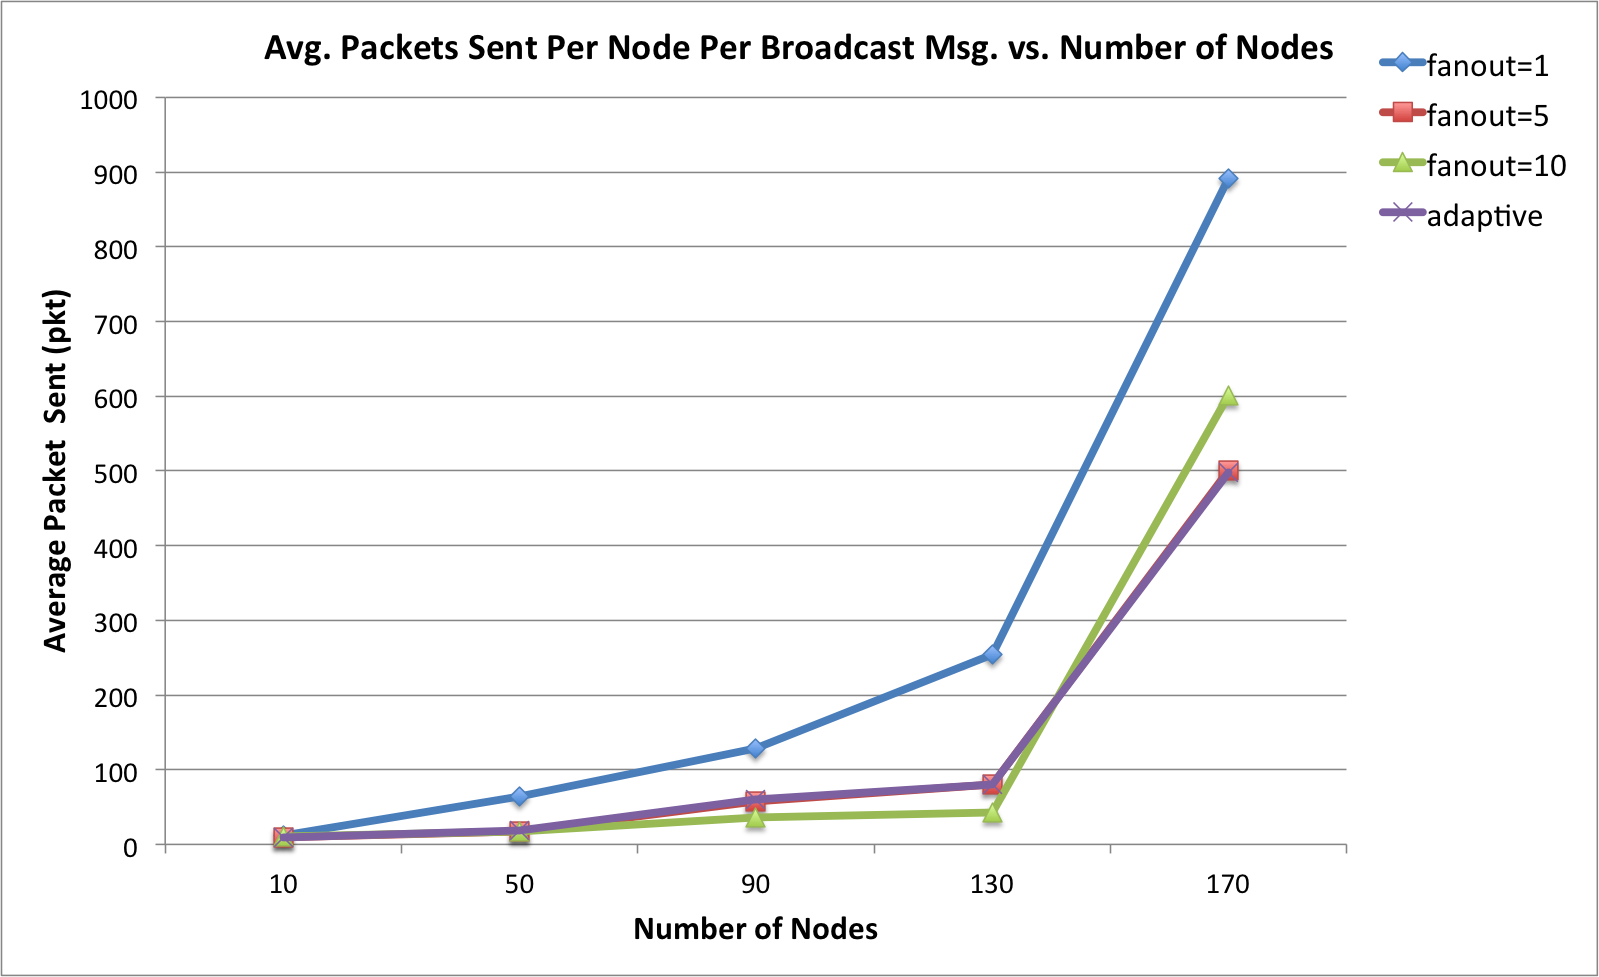
\includegraphics[width=5.5in]{overhead.png}
	\caption{Average packets sent per node per message vs. number of nodes}
	\label{fig:overhead}
\end{figure}

\begin{figure}
	\centering
	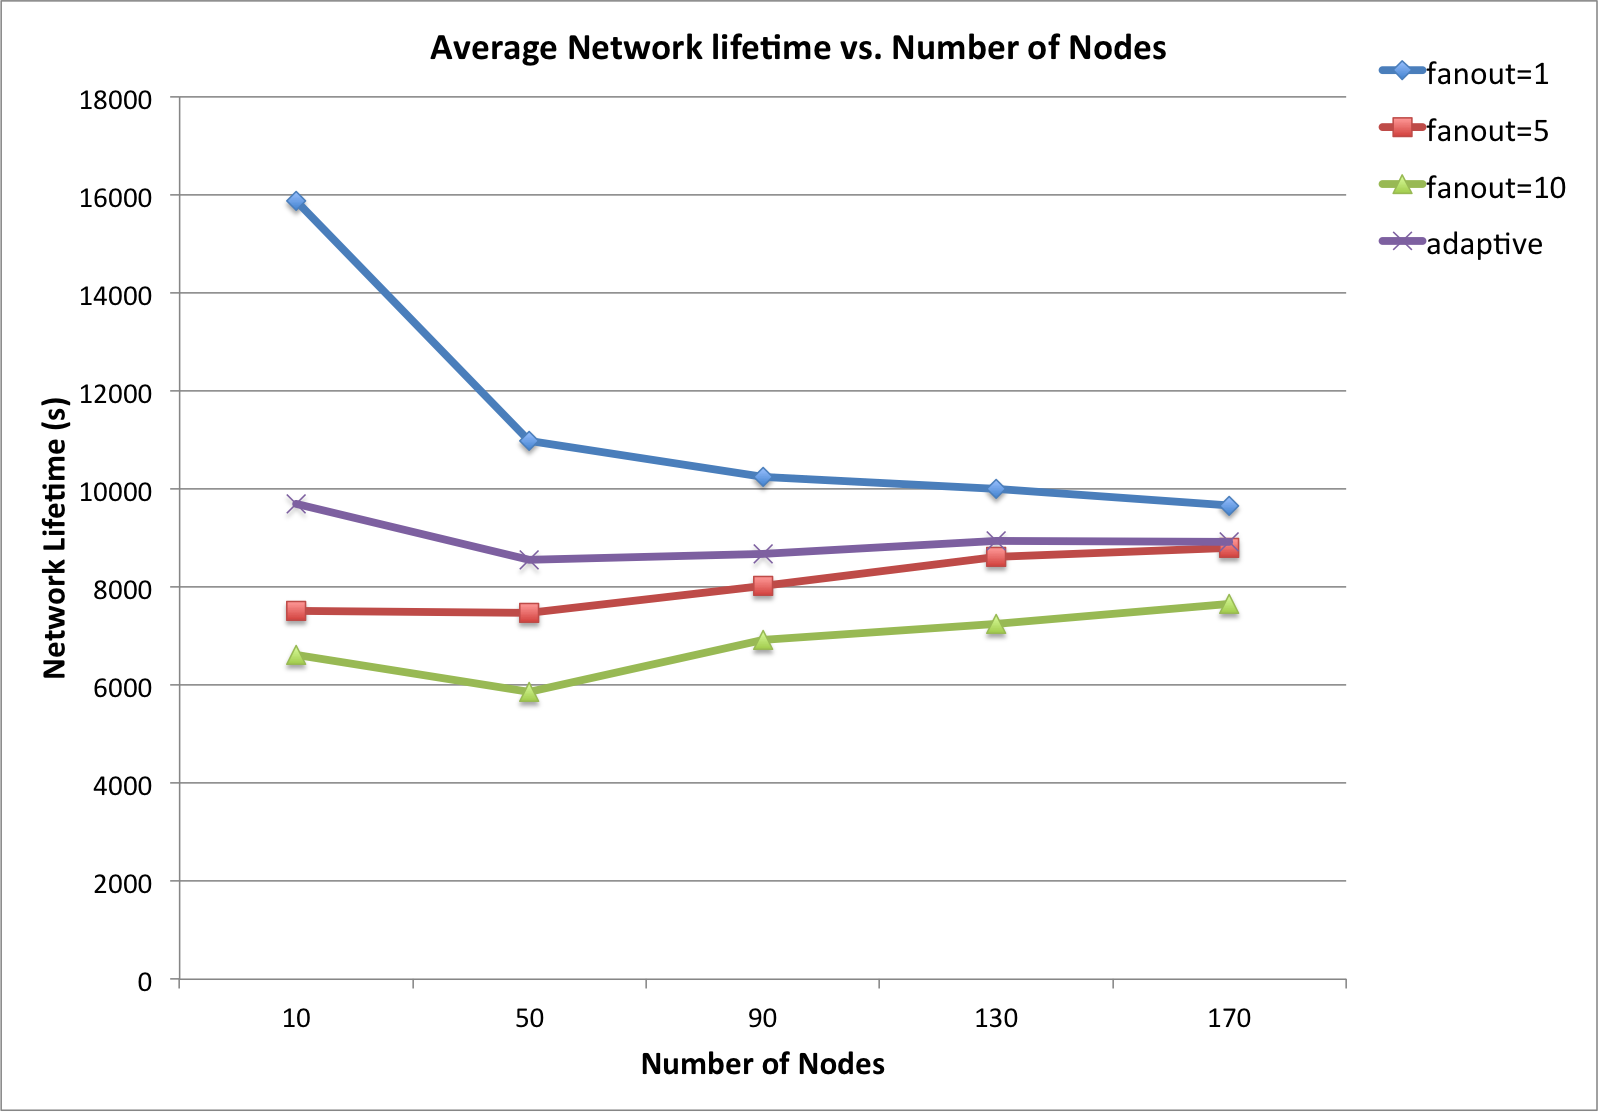
\includegraphics[width=5.5in]{life.png}
	\caption{Average network lifetime vs. number of nodes}
	\label{fig:life}
\end{figure}





(from 563 paper).

The random generated topology files are the input of our simulations. There are 7 different cases where the number of nodes vary from 100 to 1000 , increasing with 150 nodes step. And for each case, we sampled 100 topology files to run the simulations.

First, I analyzed the average number of data packets each node sent, depicted in fig.~\ref{fig:msgAbs}. It is important to note that the the collected average number for one topology file was again averaged over all reported values produced by topology files with the same number of nodes. Thus, the error bar is an indicator how consistent the average number is. It can be deduced from fig.~\ref{fig:msgAbs} that this value is ranging from 190 data packets per node to 280 data packets per node depending on the scale of the network. But considering the network scale, average number of data packets per node didn't increase proportionally as we can see in fig.~\ref{fig:msgOver}. This metrics actually decreased exponentially. 


Since when I collected the different data (average ICMP messages per node) from wired peer-to-peer network environment, here I could not perform a fair comparasion between these two evnironment. But as you can see in fig.~\ref{fig:msgP}, the average ICMP messages per node is significantly lower than in the wireless ad-hoc network. I believe the reason behind this is the shared medium for wireless communication. With shared medium, collision is prone to occur thus RTS/CTS plays an important role during the whole communicating process. Thus higher average data packets sent per node is expected.

Second, the average number of hops per node is analyzed. This is different from what we collected in the P2P environment which is maximum number of hops. Thus fair comparison between these two environment can not be performed here. In the wireless ad-hoc network, as we can see in fig. ~\ref{fig:hop}, the average number of hops per node mostly concentrated around 2.3 hops regardless of the growing number of nodes. For wired P2P network, the maximum hops is around 16.5. But the standard deviation has the tendency to decrease which is a positive sign since we hope the gossip protocol performance metrics would converge as the network grows. Nonetheless, the overall impression for both network environment is that the number of hops either average or maximum are more or less constant. But why is that the average hops per node could remaine 2 to 3 in a wireless ad-hoc network? My explaination is that since the topology of the network is almost a complete graph as you can see in fig.~\ref{fig:graph} showing a simple 10 nodes case, with gossip interval 5ms and request interval 5s, before any node send out request packets, chances are the starting node already gossipped with most of the node in the network result to a low average hops per node.

%\begin{figure}
%	\centering
%	\includegraphics[width=3in]{figs/hop}
%	\caption{The average number of hops per node (Ad-hoc environment).}
%	\label{fig:hop}
%\end{figure}
%


Moreover, figure~\ref{fig:time} illustrates the time needed to spread the message across the whole network. For the P2P network environment, the average time needed to spread the message is found to be more or less constant and slightly less than 15s. Due to the huge difference in the gossip-interval-time (5ms) and solicit-interval-time (5s), only the influence of the solicit-interval can be deduced from the results. One can see, that the time needed to spread the message is fluctuating due to the random nature of the gossip protocol, especially for the case of a number of nodes of 100, where the standard deviation is the largest. However, when we compare this result with ad-hoc network simulation result, the different between them is significant. For the latter case, the spread time starts around 190s and grows almost linearly with the number of nodes in the network. In term of absolute maginitude, wireless network perform much worse than P2P network. However, this result is total within our expectation since wireless communication often encounter collision problem and thus result in longer spread time.